\begin{figure}[!htbp]
  \centering
  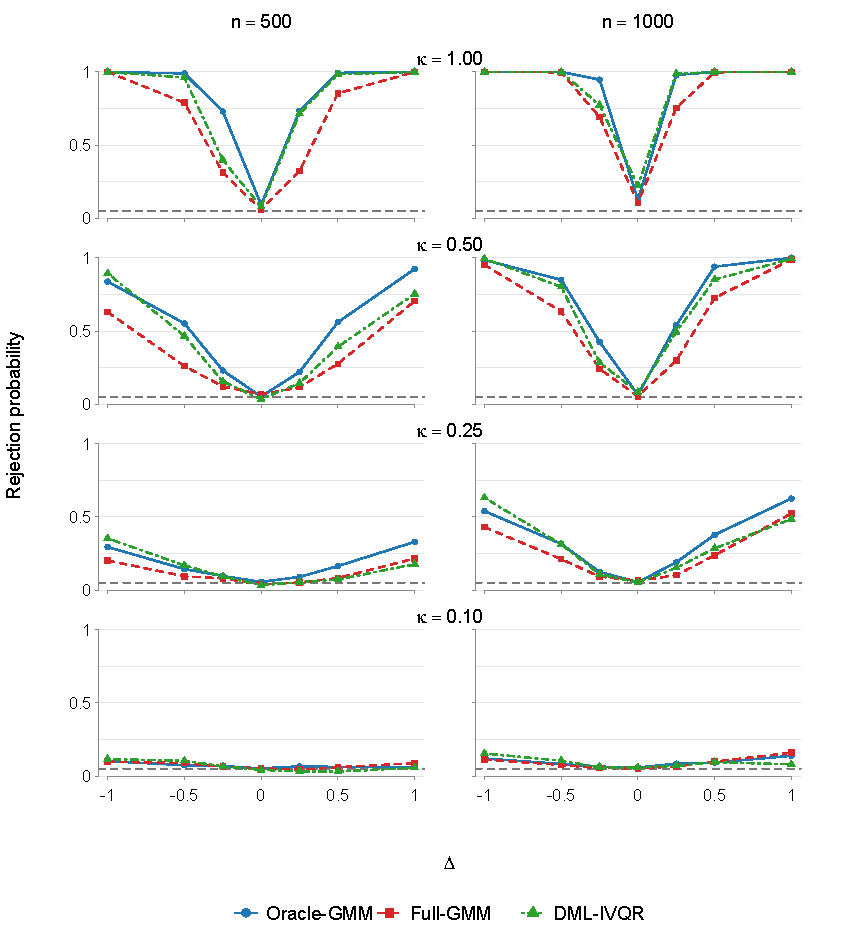
\includegraphics[width=\linewidth]{figures/generated/power_median_combined.pdf}
  \caption{Empirical power at the median.}
  \label{fig:power-median-combined}
  \begin{figurenotes}
    The median benchmark is $\tau=0.50$. Columns show $n=500$ and $n=1000$; rows show $\kappa=1.00,0.50,0.25,0.10$. The horizontal axis is $\Delta=a-\alpha_0(0.50)$, the saved deviation of the tested candidate from truth. Each point uses 500 complete replications and the same nominal 5\% chi-square cutoff; dashed horizontal lines mark 0.05. Rejection at truth is evaluated directly. At $\Delta=0$, rejection probability measures empirical size; at nonzero deviations, it measures power. These rejection probabilities are not size-adjusted. Straight segments are visual guides between evaluated points.
  \end{figurenotes}
\end{figure}
